
\section{Identification of the engine}
\subsection{Theoretical model of the DC engine}
The first step of the entire proces is determining the ideal theoretical behavior of the motors. This behavior is based on the idealised internal construction of the DC-motor and can be viewed in figure \ref{fig:DC-motor_elektrisch}. To be able to write down the transfer function of the system, the equations that govern this electrical system need to be written down. From the manipulation of these equations it is possible to get the transfer function. The obtained functions are based on the very basic equations that govern an electical system: the laws of Kirchoff. The following equations are obtained.
\begin{figure}
    \centering
    \includegraphics[scale=0.8]{{"pics assignment 1/DCmotor_el"}}
    \caption{Electrical scheme of a DC motor}
    \label{fig:DCmotor}
\end{figure}
\begin{equation}
\label{eq:kirchoff}
\begin{split}
    V_{a} - R_{a}i - L_{a}\frac{di}{dt} - V_{c} = 0 \\
    V_{c} = K_{1} \omega \\
    J\frac{d\omega}{dt} + f\omega = K_{2}i
\end{split}
\end{equation}
With
\begin{itemize}
    \item $K_{1}$ = back emf constant 
    \item $K_{2}$ = torque constant
    \item f = friction coëfficient of the engine [$\frac{Nm}{\frac{rad}{s}}$]
    \item J = Inertia of the rotor
\end{itemize}
By converting these functions to the s-domain and the use of a bit of mathematical wizardry, the theoretical transfer function obtained (cfr. eq \ref{eq:theoretische transferfunctie}). This transfer function uses the voltage source given by the arduino board ($V_{a}$). The output is the rotational speed of the engine ($\omega$). The transfer function of these in- and outputs is then
\begin{equation}
\label{eq:theoretische transferfunctie}
    \frac{\omega}{V} = \frac{K_{2}}{L_{a}Js^2 + (L_{a}f + R_{a}J)s + R_{a}f+K_{1}K_{2}}
\end{equation}
From this transfer function the poles and zeros can be calculated. The poles of the system are the s values for which the transfer function goes to infinity, so the values for which the denominator becomes zero. The zeros are the values for which the transfer function becomes zero, so the values for which the numerator is zero. It is easy to see that this specific function has no zeros. The poles can be easily calculated by solving the second degree equation. The obtained values are then

\begin{itemize}
\label{it:polen van het systeem}
    \item $s_{1}$ = $\frac{-(L_{a}f+R_{a}J) + \sqrt((L_{a}f+R_{a}J)^2-4L_{a}JK_{1}K_{2})}{L_{a}J}$
    \item $s_{2}$ = $\frac{-(L_{a}f+R_{a}J) - \sqrt((L_{a}f+R_{a}J)^2-4L_{a}JK_{1}K_{2})}{L_{a}J}$
\end{itemize}

\\
The input of the system is the voltage that is connected to the engine and is determined by the arduino program/board. The unit of the input is volt. The output is the angular velocity of the engine and its unit is rad/s. The states are angular velocity [rad/s] and electrical current [A].\\
\\
To make life easier certain effects of the engine can be neglected: the value of the coil ($L_{a}$) because it is small compared to the other values in the system. After this change the following transfer function is obtained.\cite{handboek}
\begin{equation}
\label{eq:transferfunctie eenvoudig}
    \frac{\omega}{V} = \frac{K_{2}}{R_{a}Js+R_{a}f+K_{1}K_{2}}
\end{equation}
With this simplified equation it is now possible to move to the next step: turning this continuous equation to a discrete one. The used method is the backward Euler method.  This is done by changing out the s for $\tfrac{z-1}{T_{s}z}$, with now z being the discrete domain variable and $T_{s}$ the time between two samples. After simplification the new time-discrete transfer function is obtained.
\begin{equation}
\label{eq:transferfunctie discreet}
    \frac{\omega}{V} = \frac{K_{2}T_{s}z}{(R_{a}J+R_{a}fT_{s}+K_{1}K_{2}T_{s})z-R_{a}J}
\end{equation}
\subsection{Transfer function of the engine itself}
In order to be able to get the real transfer function of the engine itself an excitation is needed. The excitation signal should be developed in such a way that it is long enough for the transient response to die out so that only the steady state response is left. A last requirement is that as many frequencies as possible have to be used.\\
\\
Taking all these requirements into account the chosen excitation signal is a block puls that starts at zero, goes up to 5 volts and back to zero. The first requirement is achieved by running the high voltage for four seconds. The second requirement is obtained by using the block puls - a block puls transformed to the frequency domain is a sinc pulse which has all the useful frequencies-. The excitition signal is shown in figure \ref{fig:excitationsignal}. On this figure the respons of the motor is also plotted. Small variations can be seen when the voltage is at it's maximum.\\
\\
During the process of applying a signal and measuring the output random noise is introduced. This noise can be minimised by repeating the signal and then overlaying these outputs. Due to this the random noise is filtered out and a clearer output signal is obtained\\
\\
\begin{figure}
    \centering
    \includegraphics[scale=0.7]{{"pics assignment 1/excitation_signal"}}
    \caption{Block puls excitation signal and the angular velocity respons}
    \label{fig:excitationsignal}
\end{figure}
In order to be able to compare the empirical system with the theoretical system they have to be of the same order. For this reason the following transfer function is chosen.
\begin{equation}
    H(z) = \frac{az}{z+b}
\end{equation}
In order to be able to write down a recursion expression, the transfer function (equation (5)) needs to be transformed to the time discrete domain. The following expression is obtained.
\begin{equation}
    y[k] = - by[k-1] + au[k]
\end{equation}
In order to make use of all the obtained data and minimise noise, the average of the responses of the five block pulses is calculated. This new data is then used to make matrix A and B. 
\begin{equation}
    B = A[b\:a]^T
\end{equation}
with
\begin{itemize}

    \item A = 
        $\begin{bmatrix}
            - y[0] & u[1] \\
            - y[1] & u[2] \\
            . & .\\
            . & .\\
            - y[k-1] & u[k]
        \end{bmatrix}$
    \item B = 
        $\begin{bmatrix}
            y[1] \\
            y[2] \\
            . \\
            . \\
            y[k]
        \end{bmatrix}$

\end{itemize}
The error criterion that minimises this expression is??\\
\\
The obtained transfer functions are then the following\\
\begin{equation}
    \frac{\omega_{A}}{V} = \frac{0.4303z}{z-0.7988}  
\end{equation}
\begin{equation}
    \frac{\omega_{B}}{V} = \frac{0.4206z}{z-0.7989}
\end{equation}
\\
Due to the low sampling frequency a lot of high frequency noise is introduced. This and other noise can be filtered out with well a filter. The chosen one in this assignment is the buttersworth filter. Another name for this filter is "maximally flat magnitude filter" which shows the first useful property of this filter: it has a uniform sensitivity for the wanted frequencies. The second useful property of this filter is that it rejects higher frequencies that are unwanted.\\
\\
The characteristics of this filter are the following. Buttersworth filter of the sixth order with a cut-off frequency of six Hz.\\
\\
After filtering the poles and zeros of the estimated transfer function have changed. The new transferfunctions are shown here.
\begin{equation}
    \frac{\omega_{A_{filtered}}}{V} = \frac{0.4945z}{z-0.7691}  
\end{equation}
\begin{equation}
    \frac{\omega_{B_{filtered}}}{V} = \frac{0.4206z}{z-0.7672}
\end{equation}
The new poles and zeros are then
\begin{itemize}
\centering
    \item $zero_{A}$ = 0
    \item $pole_{A}$ = 0.7691
    \item $zero_{B}$ = 0
    \item $pole_{B}$ = 0.7672
\end{itemize}
Figure \ref{fig:poles and zeros} shows the poles and zeros of the system before and after the filtering of the data.
\begin{figure}
    \centering
    \includegraphics[scale=0.7]{{"pics assignment 1/Poolmap_filtervsUnfilter"}}
    \caption{The poles and zeros of the transfer functions before (blue) and after (red) filtering of motor A}
    \label{fig:poles and zeros}
\end{figure}
\\
After these calculations there are three responses: the response of the motor itself (the empirical data), the non filtered data and the last being the filtered data. All three of these responses of motor A are shown in figure \ref{fig:bodetfmotorA} and the same ones of motor B are shown in figure \ref{fig:bodetfmotorB}. \\

\begin{figure}
    \centering
    \includegraphics[width=\linewidth, height=5cm]{{"pics assignment 1/transfer_MotorA"}}
    \caption{Bode plot of the different transferfunctions of motor A}
    \label{fig:bodetfmotorA}
\end{figure}
\begin{figure}
    \centering
    \includegraphics[width=\linewidth, height=5cm]{{"pics assignment 1/transfer_MotorB"}}
    \caption{Bode plot of the different transferfunctions of motor B}
    \label{fig:bodetfmotorB}
\end{figure}
\\
To validate the model a step input is used on both the actual engine and on the transfer function (based on the filtered signals) and its response is then measured. To be able to compare the output of both transfer functions, the input has to be the same. The step function in matlab can be simulated by the command lsim(). Both outputs and the difference for motor A are given in figure \ref{fig:stepresponsA}, the same is given for motor B in figure \ref{fig:stepresponsB}. In the beginning there is a huge transient difference. This difference can be attributed to the inertia of the wheel and also that it takes two time steps before voltage is given to the wheels. The differences in the steady state are very small so the estimated and simplified transfer function can be assumed to be close enough to the actual system.\\

\begin{figure}
    \centering
    \begin{minipage}[b]{0.4\linewidth}                                          \includegraphics[scale=0.4]{{"pics assignment 1/step_MotorB"}}
        \caption{Simulated and meaured respons of motor A and the difference}
        \label{fig:stepresponsA}
    \end{minipage}
    \begin{minipage}[b]{0.4\linewidth}
        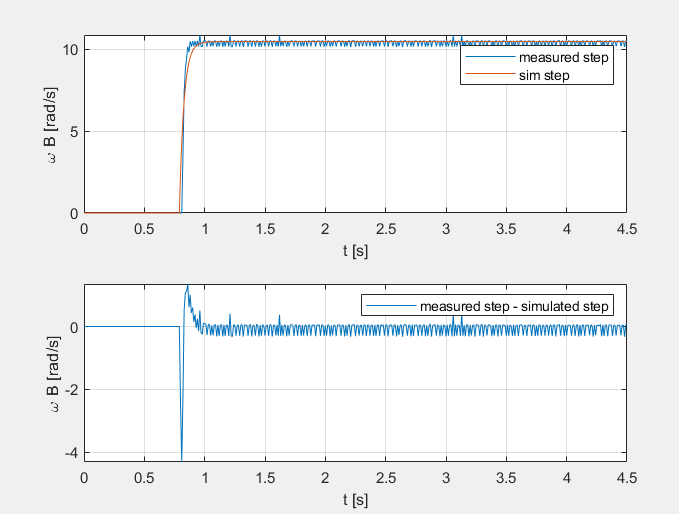
\includegraphics[scale=0.4]{{"pics assignment 1/step_MotorB.PNG}}
        \caption{Simulated and meaured respons of motor B and the difference}
        \label{fig:stepresponsB}
    \end{minipage}
\end{figure}

The superposition principle states that the output of two or more inputs has to be the sum of the responses of these inputs individually. Any function that fulfils these properties is a linear function. The formula form of this principle is the following.
\begin{equation}
    F(ax_{1}+bx_{2}) = aF(x_{1}) + b F(x_{2})
\end{equation}
In this case the different inputs (x) are the voltages applied to the motor and the outputs (F) are the speed of the wheels. 
\\
\\
To see if the transfer function fulfils this principle first an impulse of 1 volt is applied to the engine and it's response is measured, the response being the rotational velocity. Then a second voltage is applied: a five volt signal. After multiplying the output of the one volt signal by five and comparing this with the output of the six volt signal a clear difference is seen. Due to this it is clear to see that the system is non linear. This is also show in figure \ref{fig:nonlin}. The reason for this non linearity are losses in the system. Since the cart is lifted of the ground during the experiment the non-linearity is not due to friction. However there are internal losses such as eddy currents and hysteresis losses that arise due to the commutation of the magnetic field in the armature. \cite{non-linearity in DC-motor}

\begin{figure}
    \centering
    \includegraphics[scale=0.5]{{"pics assignment 1/proof_nonlinear"}}
    \caption{Proof of the non linearity of the system}
    \label{fig:nonlin}
\end{figure}



\subsection{Identification of the cart}
All the previously obtained transfer functions were determined when the wheels were freely spinning in the air. The cart however has to drive on the ground. The obtained model has to be re-evaluated with now the cart on the ground. The validation is done by the same method as before: comparing the output of a step function applied on the cart on the ground and the output of the simulated response of the derived transfer function excited by the same step input. The result is show in figure \ref{fig:groundvsair}.

\begin{figure}[h]
    \centering
    \begin{minipage}[b]{0.4\linewidth}                                          \includegraphics[scale=0.4]{{"pics assignment 1/step_wagen_grond_MotorA"}}
        \caption{measured and simulated response of motor A on the ground}
        \label{fig:stepresponsA}
    \end{minipage}
    \begin{minipage}[b]{0.4\linewidth}
        \includegraphics[scale=0.4]{{"pics assignment 1/step_wagen_grond_MotorB"}}
        \caption{measured and simulated response of motor B on the ground}
        \label{fig:stepresponsB}
    \end{minipage}
\end{figure}

The response of the cart on the ground is different to the simulated response. The reason for this is that now the tyres make contact to the ground and friction is introduced. A second reason is that now the inertia and weight of the cart influence the wheels. For this reason the response of the cart on the ground rises slower than the simulated response of the wheels in the air.\\
\\
The model now has to be re-evaluated. New data is obtained by placing the cart on the ground and applying the same block pulse that was used to identify the respons of the engine when the wheels were lifted of the ground (cfr. fig \ref{fig:excitationsignal}).\\
\\
After using this new data in the matlab code and after filtering, new transfer functions are obtained.
\begin{equation}
    \frac{\omega_A}{V} = \frac{0.05855}{z - 0.9704}
\end{equation}
\begin{equation}
    \frac{\omega_B}{V} = \frac{0.05867}{z - 0.9702}
\end{equation}
The poles and zeros of this function are
\begin{itemize}
\centering
    \item $pole_{A}$ = 0.9704
    \item $zero_{A}$ = 0
    \item $pole_{B}$ = 0.9702
    \item $zero_{B}$ = 0
\end{itemize}
A good engineer always tries to reason what will happen when inputs are changed and then sees if the output of the program matches the expectations. When placing the cart on the ground it is logical to assume that the response will be slower due to the inertia and friction. When looking at the new respons this change is clearly visible.
